\documentclass[tikz,border=2pt]{standalone}
\usepackage{amsmath,amssymb}
\usepackage{tikz}
\usetikzlibrary{arrows.meta}

\begin{document}
% Powers of z = 1.25 e^{i pi/6}: the modulus grows like r^n and the argument grows like
% n phi, so the powers spiral outwards.
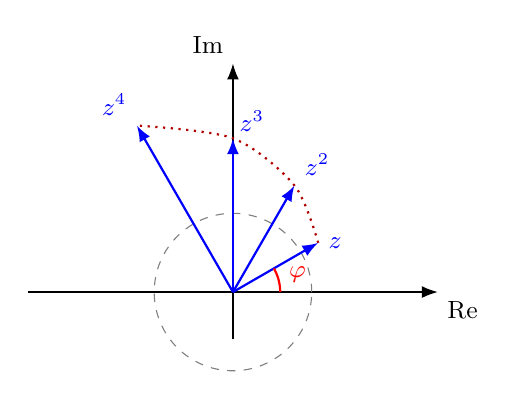
\begin{tikzpicture}[every node/.style={font=\small}, >={Latex[length=2mm]}]
	\draw[->] (-2.6,0) -- (2.6,0) node[below right] {$\mathrm{Re}$};
	\draw[->] (0,-0.6) -- (0,2.9) node[above left] {$\mathrm{Im}$};
	\draw[gray, dashed] (0,0) circle (1);
	\draw[->, blue, thick] (0,0) -- (30:1.25) node[right] {$z$};
	\draw[->, blue, thick] (0,0) -- (60:1.5625) node[above right] {$z^2$};
	\draw[->, blue, thick] (0,0) -- (90:1.953) node[above right, inner sep=2pt] {$z^3$};
	\draw[->, blue, thick] (0,0) -- (120:2.441) node[above left] {$z^4$};
	\draw[red!70!black, dotted, thick] plot[smooth] coordinates {(30:1.25) (60:1.5625) (90:1.953) (120:2.441)};
	\draw[red, thick] (0.6,0) arc (0:30:0.6);
	\node[red, font=\small] at (15:0.85) {$\varphi$};
\end{tikzpicture}
\end{document}
